\documentclass[tikz,border=5pt]{standalone}
\usepackage{luatexja}
\usepackage[hiragino-pron]{luatexja-preset}
\usepackage{amsmath,amssymb}
\usetikzlibrary{arrows.meta}

\tikzset{
  axis/.style={-{Stealth[length=6pt]}, thick},
}

% 3D to 2D projection:
%   1 unit X -> screen (-0.8, -0.5)
%   1 unit Y -> screen (1.5, 0)
%   1 unit Z -> screen (0, 1.0)
\newcommand{\projx}[3]{{-0.8*(#1)+1.5*(#2)}}
\newcommand{\projy}[3]{{-0.5*(#1)+1.0*(#3)}}

\begin{document}
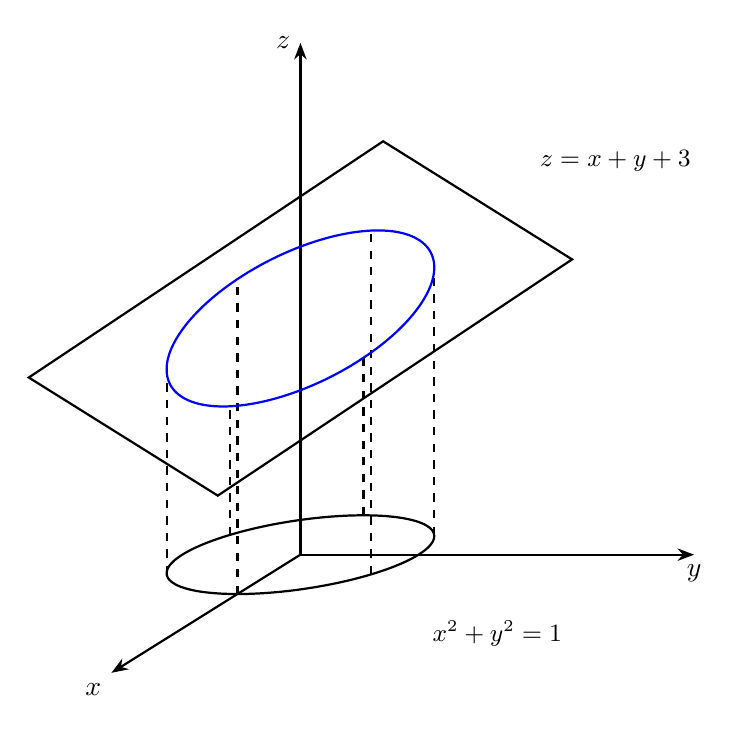
\begin{tikzpicture}[>=Stealth]

  % Axes
  \draw[axis] (0,0) -- (-2.4,-1.5) node[below left] {$x$};
  \draw[axis] (0,0) -- (5,0) node[below] {$y$};
  \draw[axis] (0,0) -- (0,6.5) node[left] {$z$};

  % Circle on xy-plane: (cos t, sin t, 0)
  % screen: (-0.8 cos t + 1.5 sin t, -0.5 cos t)
  \draw[thick] plot[domain=0:360, samples=80, smooth cycle]
    ({\projx{cos(\x)}{sin(\x)}{0}}, {\projy{cos(\x)}{sin(\x)}{0}});
  \node[font=\small] at (2.5,-1.0) {$x^2 + y^2 = 1$};

  % Dashed vertical lines at selected angles
  \foreach \t in {0, 60, 120, 180, 240, 300} {
    \draw[dashed, thick]
      ({\projx{cos(\t)}{sin(\t)}{0}}, {\projy{cos(\t)}{sin(\t)}{0}})
      --
      ({\projx{cos(\t)}{sin(\t)}{cos(\t)+sin(\t)+3}},
       {\projy{cos(\t)}{sin(\t)}{cos(\t)+sin(\t)+3}});
  }

  % Tilted plane z = x + y + 3 (draw a quadrilateral)
  \draw[thick]
    ({\projx{-1.5}{-1.5}{-1.5+(-1.5)+3}}, {\projy{-1.5}{-1.5}{-1.5+(-1.5)+3}})
    -- ({\projx{1.5}{-1.5}{1.5+(-1.5)+3}}, {\projy{1.5}{-1.5}{1.5+(-1.5)+3}})
    -- ({\projx{1.5}{1.5}{1.5+1.5+3}}, {\projy{1.5}{1.5}{1.5+1.5+3}})
    -- ({\projx{-1.5}{1.5}{-1.5+1.5+3}}, {\projy{-1.5}{1.5}{-1.5+1.5+3}})
    -- cycle;
  \node[font=\small] at (4.0,5.0) {$z = x + y + 3$};

  % Blue ellipse on the plane: (cos t, sin t, cos t + sin t + 3)
  \draw[blue, thick] plot[domain=0:360, samples=80, smooth cycle]
    ({\projx{cos(\x)}{sin(\x)}{cos(\x)+sin(\x)+3}},
     {\projy{cos(\x)}{sin(\x)}{cos(\x)+sin(\x)+3}});

\end{tikzpicture}
\end{document}
